% Hessian backpropagation scheme for a general feedforward network

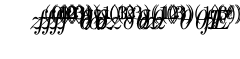
\begin{tikzpicture}
    % first four layers
    \node (in1)
        [inner sep=0]
        {\tikz \drawMessagesWithArrows{$z^{(0)}$}{ }{ }{\hNodeDistance};};
    \node (layer1)
        [anchor=south west, inner sep=0]
        at (in1.south east)
        {\tikz \drawModuleWithParams{$f^{(1)}$}{16}{$\theta^{(1)}$}{$\delta \theta^{(1)}$}{$\HeCal \theta^{(1)}$};};
    \node (out1)
        [inner sep=0, anchor=south west]
        at (layer1.south east)
         {\tikz \drawMessagesWithArrows{$z^{(1)}$}{$\delta  z^{(1)}$}{$\HeCal  z^{(1)}$}{\hNodeDistance};};
    \node (layer2)
        [inner sep=0pt, anchor=south west]
        at (out1.south east)
        {\tikz\drawModuleNoParams{$f^{(2)}$}{5};};
    \node (in2)
        [inner sep=0, anchor=south west]
        at (layer2.south east)
        {\tikz \drawMessagesWithArrows{$z^{(2)}$}{$\delta z^{(2)}$}{$\HeCal  z^{(2)}$}{\hNodeDistance};};
    \node (layer3)
        [anchor=south west, inner sep=0]
        at (in2.south east)
        {\tikz \drawModuleWithParams{$f^{(3)}$}{16}{$\theta^{(3)}$}{$\delta \theta^{(3)}$}{$\HeCal \theta^{(3)}$};};
    \node (out3)
        [inner sep=0, anchor=south west]
        at (layer3.south east)
        {\tikz \drawMessagesWithArrows{$z^{(3)}$}{$\delta  z^{(3)}$}{$\HeCal  z^{(3)}$}{\hNodeDistance};};
    \node (layer4)
        [inner sep=0pt, anchor=south west]
        at (out3.south east)
        {\tikz\drawModuleNoParams{$f^{(4)}$}{5};};	
    \node (dots)
        [xshift=2ex, inner sep=0pt, anchor=west]
         at (layer4.east) {$\dots$};

    % layer after dots
    \node (layer5)
        [xshift=12ex, anchor=south west, inner sep=0]
        at (out3.south east) 
        {\tikz \drawModuleWithParams{$f^{(\ell)}$}{16}{$\theta^{(\ell)}$}{$\delta \theta^{(\ell)}$}{$\HeCal \theta^{(\ell)}$};};
    \node (out4)
        [inner sep=0, anchor=south west]
        at (layer5.south east)
        {\tikz \drawMessagesWithArrows{$z^{(\ell)}$}{$\delta  z^{(\ell)}$}{$\HeCal  z^{(\ell)}$}{\hNodeDistance};};

    % loss layer
    \node (lossLayer) [inner sep=0pt, anchor=south west]
        at (out4.south east)
        {\tikz\drawModuleNoParams{$E$}{5};};
    \node (loss)
        [inner sep=0, anchor=south west]
        at (lossLayer.south east)
        {\tikz \drawMessagesWithArrows{$E$}{ }{ }{\hNodeDistance};};	
\end{tikzpicture}
